\chapter{INTRODUCTION}
\section{Overview}

Information organisation and management is an essential and inevitable part of everyday computer usage. Huge amount of data is produced on daily basis. With data growing in size, we are faced with the problem of locating files. Traditional file systems impose a  hierarchical structure of storage on the user. Traditional file systems are mono-hierarchical and implement directory trees to categorise and store files. In such systems, directories are the only means to access particular files.

In such systems, directories are the only means to access particular files. The path of a file contains directories, which refer to its context and categorisation. As an example \textit{``c:$\backslash$photos$\backslash$collegetrip$\backslash$museum*.jpg''} refers to all photos of a museum from a college trip. In this case, it is not possible to store that photo in another directory say \textit{``c:$\backslash$ photos$\backslash$museum*.jpg''} without copying the file. This severely limits the searching capabilities in a file system. The user is faced with the dilemma of which directory best represents the context of current file. While storing the file is identified by its file name alone which serves as its identifier. For searching a particular file, the user has to accurately remember the path and file name.

A file cannot be searched by any other information relating to its context. Creating the directory structure is based on the users organisational skills. Searching or browsing through someone else data is tricky as the organisation is different for every user. Previous approaches to such problems provided symbolic links and aliases as an incomplete answer. Symbolic links become redundant when the target file paths are changed. Similarly, aliases may become redundant or may not function properly with certain programs. Working with such solutions requires advanced skills on the users part. Keyword based searches which extract metadata from files were brought to fore by Apple's Spotlight\cite{SPOTLIGHT} and Google's Desktop Search\cite{GOOGLEDESKTOP} . Both function only on limited file types and do not allow manual categorisation. This led to the development of semantic file systems, containing categorisation of files based on context. It provides access to files by using categories formed from extracting metadata. It is similar to how music files can be searched by artist, genre, album etc. However, this presents a limitation on the amount and capabilities of what metadata can be extracted from a file. Virtual directories are used to represent data from the file system. These directories do not have a permanent listing and the user has to explicitly query for data. There have been several implementations based on semantic file systems.

However, they have several limitations in usability. Most of the projects are based only on a few key points, such as limitations over file types. This project thus is to create a semantic solution to the problems and shortcomings of traditional file systems while covering the limitations of other implemented projects.

\section{Brief Introduction}
Organising and retrieving information accurately and efficiently has attracted a lot of attention. While few have been successful, a number of innovative implementations have emerged. KWEST is a virtual file system capable of storing semantics with which it facilitates the finding of relevant information. Information is stored in tags, which are extracted from a files metadata. This information may be generated implicitly by the system or supplied explicitly by the user. Thus, the validity of information is based on the user's level of organising things.

The current system can extract metadata from a limited set of known file types. However, the modular architecture allows for plugins to be added which can add functionality for other file types. This allows for the project to be extended and modified according to the functionality required. The level of awareness generated by the system is based on the frequency of access and input provided by the user. The amount of relevance is determined by the tags generated and their associated files. This affects how the system categorises and searches files. Thus the actual outcome of the system which is the searching capabilities is totally dependent on these relationships. The current implementation is based on the Linux kernel. Future implementations can be extended to other platforms and devices. Furthermore, as the system is a virtual one, it needs only slight modifications to be ported to other file systems and operating systems.

\section{Problem Definition}
The goal of this project is to develop a semantic file system that extracts metadata from files and allows storage and searching based on its context. Such a system should overcome the drawbacks of traditional file systems while leveraging the limitations of other such similar implementations.
		
\section{Feasibility Study}
\subsection{Technical Feasibility}
The team have knowledge of C and Object Oriented concepts. The Project is being implemented using loadable kernel module known as FUSE. In the current versions of some Linux based OS this module is included in the kernel itself.
The query processing and programming will be done using SQLite. It is a relational database contained in a small C programming library. In contrast to other database management systems, SQLite is not a process that is accessed from the client application, but an integral part of it. This is also open source and is freely available.
Thus, the cost for developing KWEST will be minimal and hence will be feasible without the need for large capital.

\subsection{Economic Feasibility}
Cost of Software: We have used open-source technologies for building our system, thus there was no software cost incurred.\\
Cost of Hardware: No hardware was required to be purchased, thus no cost was incurred in building the system.
\section{Application of a Software Engineering Approach}
We are using incremental model of Software Development Life Cycle. The Software development life cycle (SDLC) is a process used by a systems analyst to develop an information system, training, and user (stakeholder) ownership. The SDLC aims to produce a high quality system that meets or exceeds customer expectations, reaches completion within time and cost estimates, works effectively and efficiently in the current and planned Information Technology infrastructure, and is inexpensive to maintain and cost-effective to enhance.The Software Development Life Cycle framework provides a sequence of activities for system designers and developers to follow. It consists of a set of steps or phases in which each phase of the SDLC uses the results of the previous one. A Software Development Life Cycle (SDLC) adheres to important phases that are essential for developers, such as planning, analysis, design, and implementation.
\begin{figure}[htb]
\centering
\setlength\fboxsep{0pt}
\setlength\fboxrule{0.5pt}
\fbox{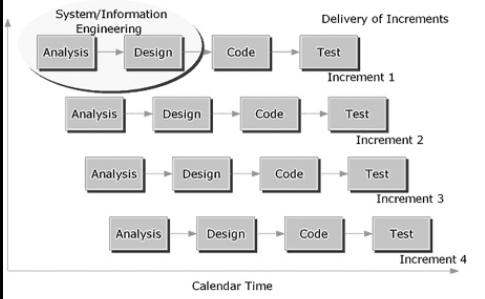
\includegraphics[width=0.75\linewidth]{./diagrams/im.png}}
%\includegraphics[width=0.8\textwidth]{image.png}
\caption{Incremental Model}
\label{fig:Im}
\end{figure}

\subsection{Planning}
During this stage, business opportunities and problems are identified, and information technology solutions are discussed. Multiple alternative projects may be suggested and their feasibility analysed.$\newline$ $\newline$ Tasks proposed were

		 \begin{enumerate}
			\item Analysing need of user to access related data.
			\item Identifying drawbacks of existing file system.
			\item The development of a project goals- identifying relations between data, file system operations, metadata storage, accessing related data.
			\item The collection of project requirements.
			\item The development of a project schedule.
			\end{enumerate}
					 
					 
\subsection{System Analysis}
The goal of system analysis is to determine where the problem is in an attempt to fix the system.This step involves breaking down the system in different pieces to analyse the situation, analysing project goals, breaking down what needs to be created and attempting to engage users so that definite requirements can be defined.$\newline$ $\newline$ Tasks proposed were


\begin{enumerate}
\item Interface for implementing file system.
\item Analyse various database alternatives based on size and speed of operation.
\item Analysis of libraries to be used for metadata operations.
\item Generation of files and tags suggestions.
\item Analysing various methods to provide user with suggestions.
\end{enumerate}
\subsection{System Design}
In systems design the design functions and operations are described in detail, including screen layouts, business rules, process diagrams and other documentation. The output of this stage will describe the new system as a collection of modules or subsystems.$\newline$ $\newline$ Tasks proposed were


				 \begin{enumerate}
				 \item Separating system implementation into following modules.
				 \item		File System Operations.
					\item	Generating Tags.
					\item	Importing Semantics.
					\item	Exporting Semantics.
					\item	Database Consistency.
				 \end{enumerate}
\subsection{Coding}
In coding we do actual implementation of system design, produced running software.$\newline$ $\newline$ Tasks proposed were


		\begin{enumerate}
		\item Implementing modules of project using finalised programming language and libraries
		\item Having modularity in code to allow for reusable modules.
			\item		Documenting the code using standard tools.
				\item		Testing project using various software testing approaches.
		\end{enumerate}
						
\subsection{Testing }
Testing is the process of evaluating a system or application, to check whether the application meets all requirements of the client and to detect the errors.$\newline$ $\newline$ Tasks proposed were


				
				\begin{enumerate}
				\item Testing of executable code using robust testing tools.
					\item Performing Regression Testing.
						\item Usability Testing.
						\item GUI Testing.
						\item Stress Testing.
						\item Integrity Testing.
				\end{enumerate}
						
\subsection{ Deployment}
Deployment starts after the code is appropriately tested, approved for release, and sold or otherwise distributed into a production environment. This may involve installation, customisation (such as by setting parameters to the customer's values), testing, and possibly an extended period of evaluation.$\newline$ $\newline$ Tasks proposed were
				\begin{enumerate}
				\item The project will be deployed as a executable which will mount the KWEST file system.
						 \item Utilise available GUI tools in the form of file managers.
						\item Installation of utility should follow standard Linux OS procedures.
		
				\end{enumerate}
						
\chapter{LITERATURE SURVEY}
Over the years, organising and retrieving information accurately and efficiently has attracted lot of attention. While few have been successful, a number of innovative implementations \cite{SEMSURVEY} have emerged. The idea of using a file's semantics as the means to categorise it has been around for quite some time. This section discusses the various
implementations made in the field of semantic file system.

An efficient implementation of keyword based searching was brought to the desktop by Apple's Spotlight\cite{SPOTLIGHT} and Google's Desktop Search\cite{GOOGLEDESKTOP} . Both allow efficient and
quick file retrieval based on keywords. They support many file types and have a simple interface which attracts a large number of users. However, both of them are limited to returning search results without any way to organising contents. In addition, they do not provide any provision to the user for classification of data. This limitation prevented the user from having a personalised way to retrieve data stored by them.

Semantic systems depend on data stored inside the files rather merely relying on an file's attributes. Most implementations use common methodologies like content recognition\cite{STAT2011} , tagging\cite{TAGFS} , extracting metadata, etc. to categorise files by using various algorithms.

``Semantic File System''\cite{SEMFS} , as developed by O'Toole and Gittord in 1992, provides
access to file contents and metadata by extracting the attributes using special modules
called ``transducers''. It was one of the very first attempts to classify files by semantics
using metadata. Its biggest drawback was the need for file type specific transducers
which were necessary to extract meta information and content from the file. Also, the
user does not have any say in what kind of category the file is classified under. This
drawback makes it an unattractive option to the general user. It was decided during
designing KWEST, that it is necessary to involve the end-user in the tagging process. This
allows each user to have their own personal way of classification and organisation of
files.

NHFS (Non Hierarchical File System)\cite{NHFS} was a project developed by Robert Freund
in July 2007. It allows the user to place any file into any number of directories. Likewise,
any directory can be placed into as many directories as required. NHFS therefore allows
one to create a non-hierarchical structure with poly-hierarchically connected files. This
allows for a powerful metaphor of finding a file in any of the category (directory) it could
be stored under. Therefore, we decided to retain this feature by using tags in place of
actual directories. Tags are associated with files and other tags as well. Thus, a tag may
be placed under multiple tags allowing a relationship to be defined between them. This
analogy is much more powerful than restricting files to actual directories. Using tags
prevents duplication and redundancy, making it an efficient implementation.

A more recent implementation is Tagsistant\cite{TAGSISTANT} , which is a semantic file system that
also attempts to organise files using tags. It interacts with the Linux kernel using the
FUSE module. Under Tagsistant, directories are considered to be equivalent to tags. As
a consequence, creating a directory is creating a tag and putting a file inside a directory
means tagging that file. After you have tagged your files, you can search all of them by
using queries. Queries are just paths where each element is either a directory or logical
operators. The entire system has a modular design and uses SQLite. However, it suffers
from some speed issues and the lack of SQL indexes. Major flaws of this design were
high consumption of inodes on real file systems and high computational time which was
required to fulfil each request. Most of the features of Tagsistant were decided to be
included in KWEST. These were modular design, SQLite repository, tagged structure, etc.
which enhance the semantics of a file system. However, care must be taken to prevent
the occurrence of similar drawbacks.

Another implementation called Tagster\cite{TAGSTER} , is a peer-to-peer tagging application for
organising desktop data. It is platform independent and is implemented in JAVA. Multiple
files and also directories can be tagged through its interface. The selected directories are
recursively examined and all files contained within them are tagged. The GUI for a Linux
system consists of three main areas.

\begin{enumerate}
 \item Tag view 
 
 It displays a list of tags.
  
\item Resource view 

 It lists resources that have the currently selected tags assigned.
\item User view

 It displays a list of users that have tagged the currently selected resource
with some selected tag. It also includes GUI support for Windows with some unresolved
issues. However, it lacks auto classification of data due to which several common tags
may be generated for each user increasing the database size.

 \end{enumerate} 

\newpage Papers referred for the developement of KWEST.
$\newline$
\begin{enumerate}
\item K. Chang, W.T. Perdana, B. Ramadhana, K. Sethuraman, T.V. Le, and N. Chachra, 
\emph{Knowledge File System-A principled approach to personal information management},
2010 IEEE International Conference on Data Mining Workshops, Sydney, December 2010, pp. 1037-1044\cite{KFS} .

$\newline$
\textit{\textbf{Abstract:}} The Knowledge File System (KFS) is a smart virtual file system that
sits between the operating system and the file system. Its primary functionality is to
automatically organise files in a transparent and seamless manner so as to facilitate
easy retrieval. Think of the KFS as a personal assistant, who can file every one of you
documents into multiple appropriate folders, so that when it comes time for you to
retrieve a file, you can easily find it among any of the folders that are likely to contain
it. Technically, KFS analyses each file and hard links (which are simply pointers to a
physical file on POSIX file systems) it to multiple destination directories (categories).
The actual classification can be based on a combination of file content analysis, file usage
analysis, and manually configured rules. Since the KFS organises files using the familiar
file/folder metaphor, it enjoys 3 key advantages against desktop search based solutions
such as Google's desktop Search, namely 1) usability, 2) portability, and 3) compatibility.
The KFS has been prototyped using the FUSE (File system in USErspace) framework
on Linux. Apache Lucene was used to provide traditional desktop search capability
in the KFS. A machine learning text classifier was used as the KFS content classifier,
complimenting the customisable rule-based KFS classification framework. Lastly, an
embedded database is used to log all file access to support file-usage classification.

		$\newline$				
		\textit{\textbf{Usefulness:}} This paper describes approach to personal information management
		through Knowledge File System. It is designed to help users organise information
		using Virtual File System to reduce the problem of manual information classification and
		retrieval. KFS provides functions so as to automatically classify the information based
		on the content similarity with respect to predefined ontologies or also give the option
		for manual classification of the information. The operations carried out on the KFS can
		also be monitored with the event logger feature. Searching of files can be carried out by
		keyword with the help of a text indexer. Furthermore the comparisons between Google
		desktop file system, beagle and KFS are given. Finally the details of the implementation
		of the KFS on the Linux platform using of FUSE are given.
		$\newline$
		\item O. Eck, and D. Schaefer, 
\emph{A semantic file system for integrated product data management}, Advanced Engineering Informatics, 2011, pp. 177-184\cite{SMFS2011} .

        $\newline$
		\textit{\textbf{Abstract:}} We initially discuss a number of disadvantages of current file management
		systems. In the body of the paper our main contribution is presented. That is, a formal
		mathematical model of a new semantic file system, SIL (Semantics Instead of Location),
		that allows engineers to access data based on semantic information rather than storage
		location is proposed. A major difference between our approach and previous related work
		is that we do not aim at yet another point solution and, instead, propose an approach that
		may be employed by next generation engineering data processing systems on a larger
		scale. In addition, a corresponding programming interface along with a graphical user
		interface used as a file browser is presented and the benefits of utilising the proposed
		semantic file system for product data management in the field of integrated design of
		mechatronic systems are discussed.
		
		$\newline$		
		\textit{\textbf{Usefulness:}} This paper describes a formal mathematical model that allows engineers
		to access data based on semantics rather than actual storage location. The main goal of
		this file system is to search files based on content of data. The browsing of the system is
		done based on file's metadata and attributes. Logical operator such as AND, OR, NOT
		are used to filter the results. The classification allows multiple tags to be created for files.
		Furthermore API's are written to create views and for the automation of notification
		updates.
		$\newline$		
		\item P. Mohan, S. Venkateswaran, Raghuraman, and A. Siromoney, 
\emph{Semantic File Retrieval in File Systems using Virtual Directories},
Proc. Linux Expo Conference, Raleigh, NC, May 2007, pp. 141-151\cite{VIRDIR} .

		$\newline$		
		\textit{\textbf{Abstract:}} Hard Disk capacity is no longer a problem. However, increasing disk capacity
		has brought with it a new problem, the problem of locating files. Retrieving a document
		from a myriad of files and directories is no easy task. Industry solutions are being created
		to address this short coming. We propose to create an extendable UNIX based File
		System which will integrate searching as a basic function of the file system. The File
		System will provide Virtual Directories which list the results of a query. The contents
		of the Virtual Directory are formed at run time. Although, the Virtual Directory is used
		mainly to facilitate the searching of file, it can also be used by plugins to interpret other
		queries.

		$\newline$				
		\textit{\textbf{Usefulness:}} This paper describes the design of SemFS, which provides semantics
		based on the file's meta-data and attributes. It allows the usage of logical operators to
		filter query results. It is implemented as a user space file system upon journaling storage.
		The architecture is server-client with support for API's to extend functionality. Features
		such as file tagging and versioning are also implemented.
		$\newline$
		\item R. Agarwal, T. Imielinski, and A. Swami, 
\emph{Mining Association Rules between Sets of Items in Large Databases}, 1993 ACM SIGMOD Conference, Washington DC, USA, May 1993, pp. 207-216\cite{MiningAssoc} .

		$\newline$		
		\textit{\textbf{Abstract :}} We are given a large database of customer transactions. Each transaction consists of 			items purchased by a customer in a visit. We present an efficient algorithm that generates all significant 					association rules between items in the database. The algorithm incorporates buffer management and novel estimation 			and pruning techniques. We also present results of applying this algorithm to sales data obtained from a large 				retailing company, which shows the effectiveness of the algorithm.

		$\newline$				
		\textit{\textbf{Usefulness :}} For finding frequently occurring file and tags, creating association rules based on 			them give and providing suggestions to user. \\ \\
		Many tagging systems exist that allow efficient manual classification of information.
		Most implementations tend to be theoretical demonstrations or complex
		implementations\cite{STMGMTSYS} existing for some very specific purpose. These suggest the
		possibility of using semantics\cite{SMO2012} in operating systems in some future date. But a
		major problem is scalability with regard to related information. However, on a large
		multi-user file system, one can get tons of tags to shift through in each folder, increasing
		the load for users to search and maintain data. Our idea is to introduce a new concept
		of relating tags to overcome this situation. Implementing all the desired and necessary
		features from previous implementations, our design goal is to create an efficient Semantic
		File System which could be used by any class of users.
		\end{enumerate}